% Provenance (never printed): see sources/outline_sources.md (Year 3:
% moments of inertia and gravity fields; impact cratering and crater dating;
% volcanism and tectonics on Mars, Venus, Io and the icy moons).
% Brief: sources/book5/BRIEFS.md, ch. 26. Curves from figdata/bachelor-3/
% two_layer_planet.py (two-layer interiors of the Earth, Mars, the Moon and
% Mercury from mean density and moment of inertia) and crater_sfd.py
% (the Ivanov production function and the Hartmann-Neukum chronology of
% Mars from the Craterstats configuration, the lunar chronology of Neukum,
% Hartmann's equilibrium density, and two invented Martian plains whose
% counts are drawn once from a Poisson law). Exercise and problem values in
% the Book 5 scratch calculator calc/ch26.py. Plains A and B are invented.
\chapter{Interior dan Permukaan Planet}\label{ch:b3:planetary-interiors-surfaces}

Dilihat dengan teropong, Bulan memiliki dua jenis permukaan. Dataran tinggi yang
terang tertutup kawah, kawah di atas kawah: pengeboman intens yang berakhir
sekitar 3.8 miliar tahun lalu telah menjenuhkannya dengan kawah-kawah besar.
Mare gelap, dataran yang terisi lava antara 4.2 dan 1.2
miliar tahun lalu, memuat jauh lebih sedikit kawah. Misi Apollo dan Luna
membawa pulang batuan dari keduanya, dan umur radiometriknya menjadikan
jumlah kawah per satuan luas permukaan sebuah jam. Jam itu kini menentukan umur
dataran di Mars, Merkurius dan bulan-bulan es, yang belum satu pun batuannya
dibawa pulang. Bab ini membaca interior planet dari gravitasinya, rotasinya,
dan pasang surutnya, lalu permukaannya lewat kawah-kawahnya,
gunung apinya, dan sesarnya.
% ledger: french:highlands, nasa:moon-core, marchi:neukum

\begin{recall}
Faktor momen inersia $C = I/MR^2$, model dua lapis planet yang dibangun darinya
dan massa jenis rata-rata, serta planet batuan dan planet raksasa, dibahas di
volume Tahun 1, dalam bab tentang
planetologi komparatif; plume mantel dan provinsi beku besar, dalam bab tentang
titik panas. Diferensiasi planet dan meteorit dibahas di volume Tahun 2,
dalam bab tentang pembentukan planet. \omterm{def:b3:gravity-geodesy:j2}{Faktor bentuk dinamis}
$J_2$, \omterm{thm:b3:gravity-geodesy:maccullagh}{rumus MacCullagh}, dan \omterm{def:b3:gravity-geodesy:flexure}{lenturan litosfer} dibahas dalam
volume ini, dalam bab tentang gravitasi dan geodesi; \omterm{def:b3:mantle-convection:rayleigh}{bilangan Rayleigh}, dalam
bab tentang konveksi mantel. Pasang surut, hukum Kepler, dan modulus elastis
dibahas di buku fisika; distribusi Poisson, di buku
matematika.
\end{recall}

\section{Interior dari gravitasi, rotasi dan pasang surut}\label{sec:b3:planetary-interiors-surfaces:interiors}

Massa planet, dari orbit bulan atau wahana angkasa, memberi massa jenis
rata-rata; presesi sumbunya dan $J_2$-nya memberi momen
inersia. Proposisi dua lapis di volume Tahun 1 mengubah kedua angka itu
menjadi inti, tetapi hanya setelah massa jenis mantel dipilih: dua pengukuran
tidak dapat menentukan tiga besaran yang tidak diketahui.

\begin{omfigure}
\centering
\begin{tikzpicture}
\begin{axis}[width=0.78\linewidth, height=0.46\linewidth,
  xmin=3000, xmax=16000, ymin=0, ymax=1,
  xlabel={kepadatan inti $\rho_c$ (\unit{kg.m^{-3}})},
  ylabel={jari-jari inti / jari-jari planet $x$},
  tick label style={font=\scriptsize}, label style={font=\small},
  scaled x ticks=false, xtick={4000,6000,8000,10000,12000,14000,16000},
  xticklabels={4000,6000,8000,10\,000,12\,000,14\,000,16\,000}]
\addplot[thick, omDef] table[x=rho_c, y=x] {figdata/out/bachelor-3-two_layer_planet-curve-Earth.dat};
\addplot[thick, red!70!black] table[x=rho_c, y=x] {figdata/out/bachelor-3-two_layer_planet-curve-Mars.dat};
\addplot[thick, black!60, dashed] table[x=rho_c, y=x] {figdata/out/bachelor-3-two_layer_planet-curve-Moon.dat};
\addplot[thick, orange!80!black] table[x=rho_c, y=x] {figdata/out/bachelor-3-two_layer_planet-curve-Mercury.dat};
\addplot[only marks, mark=*, mark size=2pt, black] table[x=rho_c, y=x] {figdata/out/bachelor-3-two_layer_planet-points.dat};
\node[font=\scriptsize, omDef, anchor=south west] at (axis cs:12600,0.55) {Bumi};
\node[font=\scriptsize, red!70!black, anchor=south west] at (axis cs:6600,0.55) {Mars};
\node[font=\scriptsize, black!70, anchor=south west] at (axis cs:11000,0.2) {Bulan};
\node[font=\scriptsize, orange!80!black, anchor=south west] at (axis cs:7300,0.83) {Merkurius};
\end{axis}
\end{tikzpicture}
\par\smallskip{\small Model dua lapis yang diizinkan oleh massa jenis rata-rata dan
faktor momen inersia empat benda: setiap kurva membentang di atas kisaran
massa jenis mantel yang mungkin, dengan mantel yang lebih rapat menyisakan inti
yang lebih kecil dan lebih rapat. Titik-titik menandai jari-jari inti terukur: milik Bumi dari seismologi,
milik Mars dari seismometer InSight, inti dalam dan kulit cair Bulan,
milik Merkurius dari medan gravitasi wahana MESSENGER
angkasa.}\label{fig:b3:planetary-interiors-surfaces:two-layer}
\end{omfigure}
% ledger: planet:Earth.density, planet:Mars.density, planet:Moon.density, planet:Mercury.density, earth:MoI, nasa:mars, nasa:moon, nasa:mercury, data:prem, jpl:insight-interior, nasa:moon-core, agu:mercury-core

Setiap planet menghasilkan kurva, bukan satu titik. Untuk Mars, jari-jari inti
\qty{1830}{km} yang diukur InSight memilih mantel dengan massa jenis \qty{3460}{kg.m^{-3}}
dan inti dengan massa jenis \qty{6460}{kg.m^{-3}}. Untuk Merkurius, inti dengan jari-jari sekitar
\qty{2000}{km} mengisi 82~persen jari-jari planet. Kurva untuk Bulan
hampir datar: nilai $C = 0.394$ sangat dekat dengan $\tfrac25$ sehingga inti kecil
dengan massa jenis berapa pun cocok, dan perubahan $0.001$ pada $C$ menggeser jari-jari inti
lebih dari dua kali lipat (\cref{exo:b3:planetary-interiors-surfaces:10}).
Gravitasi saja tidak dapat melihat inti kecil; pasang surut dan gelombang seismik dapat.
% ledger: jpl:insight-interior, agu:mercury-core, nasa:moon

\begin{definition}[bilangan Love]\label{def:b3:planetary-interiors-surfaces:love-number}
Ketika potensial pasang surut berderajat~2 bekerja pada planet, planet itu berdeformasi dan
massa yang terdistribusi ulang menambahkan potensialnya sendiri. Yang disebut \emph{bilangan
Love}\index{bilangan Love} $k_2$ adalah rasio potensial tambahan itu terhadap
potensial pasang surut, keduanya diambil di permukaan planet.
\end{definition}

Planet kaku memiliki $k_2 = 0$; planet fluida bermassa jenis seragam merespons
sepenuhnya, dengan $k_2 = \tfrac32$. Di antara keduanya, angka itu mengukur seberapa
banyak bagian planet yang mengalah.

\begin{proposition}[Bilangan Love dari bola elastis seragam]\label{prop:b3:planetary-interiors-surfaces:kelvin}
Bola tak termampatkan dengan massa jenis seragam $\rho$, jari-jari $R$, gravitasi permukaan
$g$, dan kekakuan $\mu$ memiliki
\[
  k_2 = \frac{3/2}{1 + \dfrac{19\mu}{2\rho g R}} .
\]
\end{proposition}

Hasil ini, dari Kelvin, diterima tanpa pembuktian. Rasio $\mu/\rho gR$ membandingkan
kekakuan elastis dengan gravitasi sendiri yang menarik tonjolan pasang surut
kembali: planet kecil bersifat kaku, planet besar mengalah. Untuk Mars, $\rho gR =
\qty{4.97e10}{Pa}$; dengan kekakuan mantel atas Bumi,
\qty{67}{GPa} pada kedalaman \qty{80}{km} dalam model acuan Bumi, rumus
memberikan $k_2 = 0.109$. Pelacakan orbiter Mars Global Surveyor
mengukur pasang surut Matahari di Mars: $k_2 = 0.153 \pm 0.017$, terlalu
besar untuk inti besi padat. Setidaknya bagian luar inti bersifat cair,
dan jari-jarinya ditetapkan antara 1520 dan \qty{1840}{km} pada 2003.
% ledger: nasa:mars, const:G, data:prem, yoder:mars-k2

Seismometer menjawab persoalan itu. Pendarat InSight merekam
gempa Mars dan mendeteksi gelombang yang dipantulkan dari puncak inti: jari-jari
\qty{1830}{km}, di bawah mantel sedalam \qty{1560}{km} dan kerak dengan tebal 20 sampai
\qty{37}{km}. Di Bulan, seismometer yang dipasang oleh astronot Apollo
merekam gempa Bulan; yang terdalam di antaranya, ratusan
kilometer ke bawah permukaan, dipicu pasang surut Bumi. Inti Bulan kini digambarkan
sebagai inti dalam padat kaya besi berjari-jari \qty{240}{km}, sebuah
cangkang besi cair setebal \qty{90}{km} yang mengelilinginya, dan lapisan
sebagian meleleh di atasnya.
% ledger: jpl:insight-interior, nasa:moonquakes, nasa:moon-core

\section{Pembentukan kawah akibat tumbukan}\label{sec:b3:planetary-interiors-surfaces:impacts}

Benda dari angkasa menumbuk planet dengan laju tidak kurang dari
kecepatan lepas planet, \qty{11.2}{km.s^{-1}} untuk Bumi; asteroid umumnya
menumbuk Bumi pada kecepatan 15 sampai \qty{25}{km.s^{-1}}, dan komet hingga
\qty{60}{km.s^{-1}}. Pada \qty{20}{km.s^{-1}} setiap kilogram membawa
\qty{2e8}{J}, sekitar lima puluh kali energi satu kilogram bahan peledak. Tumbukan
mengirimkan gelombang kejut ke dalam tanah dan proyektil, yang
meleleh dan menguap; di belakang gelombang kejut batuan mulai bergerak keluar, dan
sebuah kawah terbentuk dalam hitungan detik.
% ledger: french:velocities, french:table21

\begin{definition}[Kawah sementara, kawah sederhana, kawah kompleks, dan selimut ejekta]\label{def:b3:planetary-interiors-surfaces:crater-morphology}
Yang disebut \emph{kawah sementara}\index{kawah sementara} adalah rongga berbentuk mangkuk
yang terbentuk oleh aliran penggalian pada saat berhenti membesar; kedalamannya
kira-kira sepertiga dari diameternya. Adapun \emph{kawah
sederhana}\index{kawah sederhana} adalah mangkuk dengan tepi terangkat, kawah sementara
hampir tidak berubah: dinding curamnya runtuh ke dalam menjadi lensa
breksi. Adapun \emph{kawah kompleks}\index{kawah kompleks} adalah kawah yang lebih besar
yang cekungan sementaranya runtuh: lantainya naik menjadi pengangkatan pusat, tepinya
meluncur ke dalam sepanjang teras, dan lantainya datar. Yang disebut \emph{selimut
ejekta}\index{selimut ejekta} adalah lapisan batuan tergali yang terlempar keluar
melewati tepi dan terendap di sekeliling kawah.
\end{definition}
% ledger: french:transient, french:transition

\begin{omfigure}
\centering
\begin{tikzpicture}[x=0.55cm, y=0.55cm, font=\scriptsize, >=stealth]
\def\simpleprofile{(-6,0) -- (-3.6,0) .. controls (-3.0,0.45) .. (-2.6,0.55) .. controls (-1.8,-2.6) and (1.8,-2.6) .. (2.6,0.55) .. controls (3.0,0.45) .. (3.6,0) -- (6,0)}
\def\complexprofile{(-7,0) -- (-5.4,0) -- (-4.6,0.5) -- (-4.0,-0.3) -- (-3.6,-0.25) -- (-3.1,-1.0) -- (-2.7,-0.95) -- (-2.3,-1.5) -- (-0.8,-1.5) -- (-0.5,-0.6) -- (0,-0.3) -- (0.5,-0.6) -- (0.8,-1.5) -- (2.3,-1.5) -- (2.7,-0.95) -- (3.1,-1.0) -- (3.6,-0.25) -- (4.0,-0.3) -- (4.6,0.5) -- (5.4,0) -- (7,0)}
\begin{scope}
\fill[black!8] \simpleprofile -- (6,-4) -- (-6,-4) -- cycle;
\begin{scope}
\clip \simpleprofile -- (6,-4) -- (-6,-4) -- cycle;
\draw[black!45] (-6,-1.2) -- (6,-1.2) (-6,-2.4) -- (6,-2.4);
\fill[black!28] (-2.25,-0.5) .. controls (-1.2,-2.05) and (1.2,-2.05) .. (2.25,-0.5) .. controls (1.0,-0.8) and (-1.0,-0.8) .. (-2.25,-0.5);
\end{scope}
\fill[black!40] (-5.2,0) -- (-2.6,0.55) -- (-3.6,0.12) -- cycle;
\fill[black!40] (5.2,0) -- (2.6,0.55) -- (3.6,0.12) -- cycle;
\draw[thick] \simpleprofile;
\draw[omDef, dashed, thick] (-2.4,0.35) .. controls (-1.6,-3.1) and (1.6,-3.1) .. (2.4,0.35);
\node[anchor=south] at (0,1.2) {kawah sederhana};
\node[fill=black!28, inner sep=1pt] at (0,-1.45) {lensa breksi};
\node[omDef, anchor=north, fill=black!8, inner sep=1pt] at (0,-2.65) {kawah sementara};
\draw[->] (-4.9,1.2) node[anchor=south] {ejekta} -- (-4.3,0.2);
\draw[->] (3.6,1.4) node[anchor=south] {tepi terangkat} -- (2.8,0.62);
\end{scope}
\begin{scope}[xshift=7.6cm]
\fill[black!8] \complexprofile -- (7,-4) -- (-7,-4) -- cycle;
\begin{scope}
\clip \complexprofile -- (7,-4) -- (-7,-4) -- cycle;
\draw[black!45] (-7,-1.2) -- (7,-1.2);
\draw[black!45] (-7,-2.4) -- (-1.3,-2.4) .. controls (-0.6,-2.4) and (-0.5,-1.75) .. (0,-1.75) .. controls (0.5,-1.75) and (0.6,-2.4) .. (1.3,-2.4) -- (7,-2.4);
\draw[black!45] (-7,-3.4) -- (-1.6,-3.4) .. controls (-0.7,-3.4) and (-0.6,-2.7) .. (0,-2.7) .. controls (0.6,-2.7) and (0.7,-3.4) .. (1.6,-3.4) -- (7,-3.4);
\draw[black!70] (-4.0,-0.3) -- (-3.2,-2.0) (4.0,-0.3) -- (3.2,-2.0) (-3.1,-1.0) -- (-2.5,-2.2) (3.1,-1.0) -- (2.5,-2.2);
\end{scope}
\draw[thick] \complexprofile;
\node[anchor=south] at (0,1.5) {kawah kompleks};
\draw[->] (1.4,0.75) node[anchor=south west, inner sep=1pt] {pengangkatan pusat} -- (0.25,-0.2);
\node[anchor=north, fill=black!8, inner sep=0.5pt] at (-1.3,-1.6) {dasar datar};
\draw[->] (-3.2,1.4) node[anchor=south] {teras} -- (-3.8,-0.12);
\draw[->] (-5.6,-0.6) node[anchor=east, fill=black!8, inner sep=1pt, xshift=4pt] {sesar} -- (-3.65,-1.35);
\node[anchor=north, fill=black!8, inner sep=1pt] at (0,-3.55) {lapisan terangkat};
\end{scope}
\end{tikzpicture}
\par\smallskip{\small Penampang lintang \omterm{def:b3:planetary-interiors-surfaces:crater-morphology}{kawah sederhana} dan \omterm{def:b3:planetary-interiors-surfaces:crater-morphology}{kawah kompleks} dalam
batuan berlapis (tidak sesuai skala). Kiri: cekungan \omterm{def:b3:planetary-interiors-surfaces:crater-morphology}{kawah sederhana} mempertahankan
bentuk \omterm{def:b3:planetary-interiors-surfaces:crater-morphology}{kawah sementara} (putus-putus), sebagian terisi lensa breksi,
di bawah tepi terangkat dan \omterm{def:b3:planetary-interiors-surfaces:crater-morphology}{selimut ejekta}. Kanan: pada \omterm{def:b3:planetary-interiors-surfaces:crater-morphology}{kawah kompleks} cekungan
sementara telah runtuh; lapisan-lapisan dalam naik di bawah pengangkatan
pusat, dan tepi meluncur ke dalam sepanjang sesar menjadi
teras.}\label{fig:b3:planetary-interiors-surfaces:craters}
\end{omfigure}
% ledger: french:transient, french:transition

\begin{omfigure}
\centering
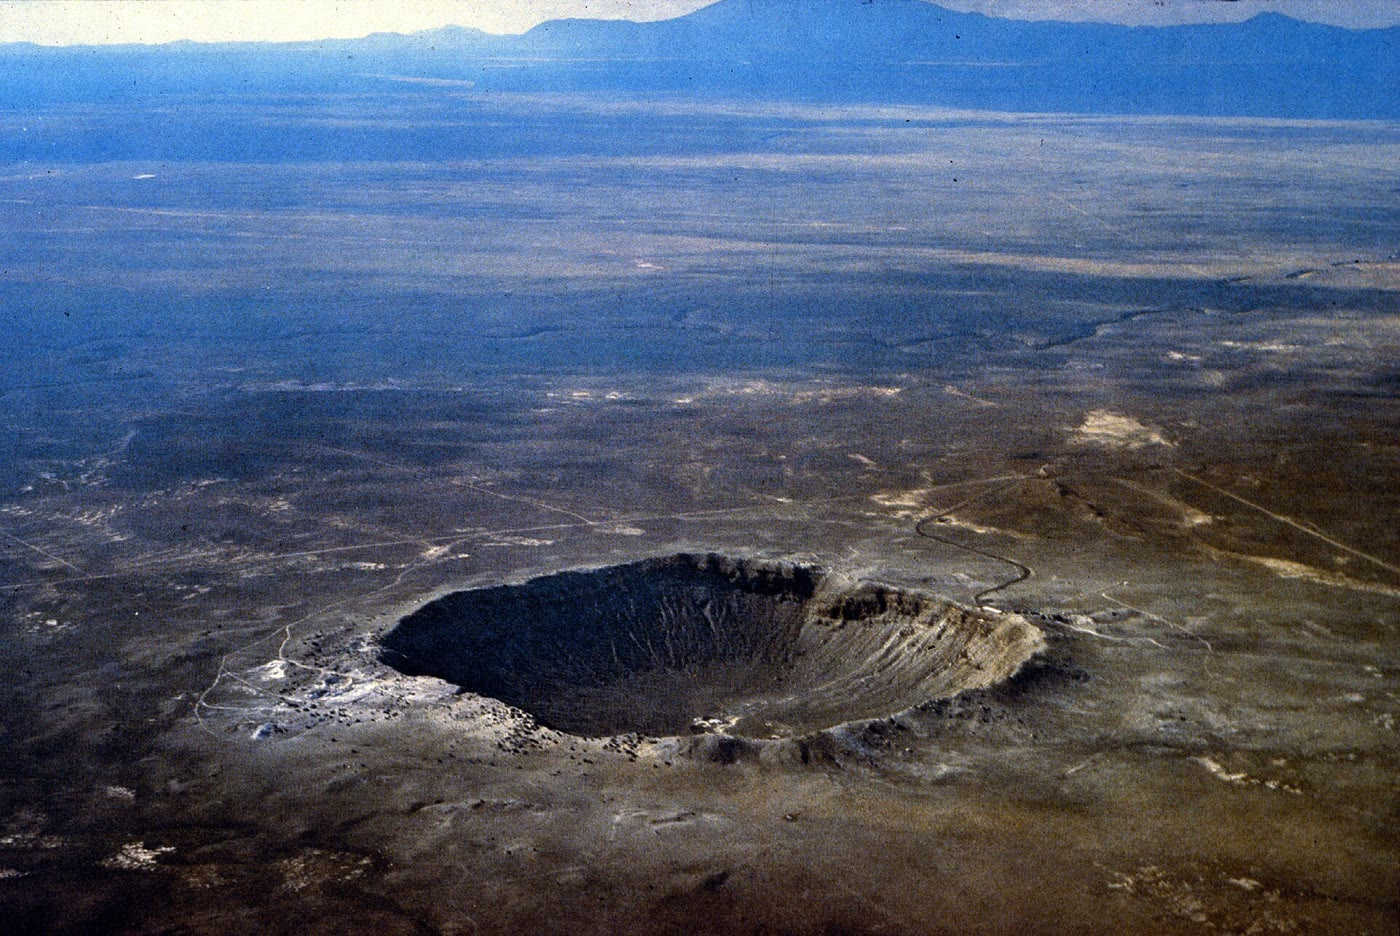
\includegraphics[width=0.66\linewidth]{images/book5/b3-barringer-crater.jpg}
\par\smallskip{\small Barringer Meteor Crater, Arizona, sebuah \omterm{def:b3:planetary-interiors-surfaces:crater-morphology}{kawah sederhana}
berdiameter \qty{1.2}{km}, terbentuk sekitar 50\,000 tahun lalu akibat meteorit besi
berukuran sekitar \qty{30}{m}; tepinya menjulang di atas dataran tinggi, dan \omterm{def:b3:planetary-interiors-surfaces:crater-morphology}{selimut ejekta}
menyebar di sekelilingnya. Foto udara, USGS/D.~Roddy, domain
publik.}\label{fig:b3:planetary-interiors-surfaces:barringer}
\end{omfigure}
% ledger: photo:b3-barringer, french:barringer

Penggalian kawah berdiameter \qty{1}{km} memerlukan sekitar enam detik, sedangkan yang
berdiameter \qty{200}{km} sekitar satu setengah menit. Ukuran kawah
yang dibentuk tumbukan bergantung pada energi proyektil, gravitasi, dan
kekuatan batuan; hukum-hukum yang menghubungkannya dicocokkan pada
eksperimen dan ledakan dalam bentuk hasil kali besaran tak berdimensi
kelompok, dan kita terima di sini. Intinya terletak pada keseimbangan energi.
% ledger: french:transient

\begin{proposition}[Penskalaan rezim gravitasi]\label{prop:b3:planetary-interiors-surfaces:scaling}
Jika suatu pecahan tetap dari energi tumbukan $E$ mengangkat batuan tergali
bermassa jenis $\rho$ melawan gravitasi $g$, diameter kawah membesar sebagai
\[
  D \propto \left(\frac{E}{\rho g}\right)^{1/4} .
\]
\end{proposition}

\begin{proof}
Volume yang tergali sebanding dengan $D^3$, massanya $\rho D^3$, dan ia
terangkat setinggi kira-kira $D$: usahanya berorde $\rho g D^4$, yang
sebanding dengan $E$.
\end{proof}

Sebagian energi berubah menjadi panas untuk melelehkan dan mematahkan batuan, sehingga
hukum yang sebenarnya berada di antara hukum ini dan aturan yang lebih sederhana: sebuah tabel
yang sering dikutip untuk Bumi memberikan kawah yang lebarnya dua puluh kali proyektil batunya.
Gravitasi juga menentukan di mana kawah berhenti menjadi sederhana. Dinding
mangkuk sementara runtuh ketika berat batuan yang ditahannya,
berorde $\rho g D/3$, melampaui kekuatan batuan, sehingga diameter transisinya
bervariasi sebagai $1/g$: kira-kira \qty{4}{km} di batuan kristalin dan
\qty{2}{km} di sedimen pada Bumi, serta kira-kira \qty{20}{km} di
Bulan, tempat gravitasinya enam kali lebih lemah.
% ledger: french:table21, french:transition, planet:Earth.gravity, planet:Moon.gravity

\section{Penanggalan kawah}\label{sec:b3:planetary-interiors-surfaces:dating}

Permukaan yang dibiarkan begitu saja mengumpulkan kawah dengan laju ketika benda-benda
menumbuknya. Dengan menghitung kawahnya, kita dapat menentukan umur permukaan itu,
asalkan laju itu diketahui dan kawah-kawahnya memang milik permukaan itu, bukan milik apa yang
terkubur di bawahnya atau puing yang terlempar dari tetangganya.

\begin{definition}[Distribusi ukuran--frekuensi kawah]\label{def:b3:planetary-interiors-surfaces:sfd}
\emph{Distribusi ukuran--frekuensi kawah}\index{distribusi ukuran--frekuensi kawah}
suatu permukaan adalah jumlah $N(D)$ kawah berdiameter paling sedikit $D$ per
satuan luas, sebagai fungsi $D$ (distribusi kumulatif), atau jumlah yang
dihitung dalam selang diameter, yang biasanya masing-masing $\sqrt2$ kali lebih
lebar daripada selang sebelumnya (distribusi inkremental).
\end{definition}

\begin{definition}[Penanggalan kawah; fungsi produksi dan kronologi; massa jenis kesetimbangan]\label{def:b3:planetary-interiors-surfaces:crater-dating}
\emph{Penanggalan kawah}\index{penanggalan kawah} adalah penentuan umur
suatu permukaan dari massa jenis kawahnya. \emph{Fungsi produksi
kawah}\index{fungsi produksi kawah} adalah bentuk \omterm{def:b3:planetary-interiors-surfaces:sfd}{distribusi ukuran--frekuensi
kawah} yang diperoleh suatu permukaan, $F(D) =
N(D)/N(\qty{1}{km})$, yang diasumsikan sama pada setiap umur. \emph{Fungsi
kronologi kawah}\index{fungsi kronologi kawah} $N_1(T)$ adalah jumlah kawah
berukuran \qty{1}{km} atau lebih per satuan luas yang terakumulasi dalam
waktu $T$. Suatu permukaan berada pada \emph{massa jenis kesetimbangan
kawah}\index{massa jenis kesetimbangan kawah} untuk kawah berukuran tertentu
ketika setiap kawah baru, rata-rata, menghapus sebanyak kawah lama yang
ditambahkannya: jumlahnya tidak lagi bertambah.
\end{definition}

\omterm{def:b3:advanced-geochronology:model-age}{Umur model} suatu permukaan diperoleh dari satu kali penghitungan: $N(D)$ yang
diukur pada sembarang $D$ memberikan $N_1 = N(D)/F(D)$, dan $T$ memenuhi
$N_1(T) = N_1$. Garis-garis $N(D) = N_1(T)F(D)$ untuk $T$ tetap disebut
isokron. Untuk Mars, fungsi produksi yang banyak dipakai adalah polinomial
berderajat~11 dalam $\log_{10}D$, dan fungsi kronologinya berbentuk
\[
  N_1(T) = a\left(e^{bT} - 1\right) + cT , \qquad
  a = \qty{3.22e-14}{km^{-2}}, \ b = \qty{6.93}{Ga^{-1}}, \
  c = \qty{4.875e-4}{km^{-2}.Ga^{-1}} ,
\]
linear selama tiga miliar tahun terakhir, sementara sebelumnya eksponensial curam.
Fungsi Bulan memiliki bentuk yang sama dengan $a = \num{5.44e-14}$ dan $c =
\num{8.38e-4}$. Fungsi ini dicocokkan dengan umur situs pendaratan Apollo dan
Luna; fungsi Mars diperoleh dari fungsi Bulan yang diskalakan dengan taksiran
rasio laju pembentukan kawah di Mars dan di Bulan.
% ledger: craterstats:mars-pf, craterstats:mars-cf, craterstats:moon-cf, marchi:neukum

\begin{omfigure}
\centering
\begin{tikzpicture}
\begin{groupplot}[group style={group size=2 by 1, horizontal sep=1.6cm},
  width=0.48\linewidth, height=0.46\linewidth,
  tick label style={font=\scriptsize}, label style={font=\small}, title style={font=\small}]
\nextgroupplot[title={isokron di Mars}, xmode=log, ymode=log, xmin=0.1, xmax=100,
  ymin=1e-8, ymax=100, xlabel={diameter kawah $D$ (\unit{km})},
  ylabel={$N(D)$, kawah $\geq D$ per \unit{km^2}},
  xtick={0.1,1,10,100}, xticklabels={0.1,1,10,100},
  ytick={1e-8,1e-6,1e-4,1e-2,1}]
\addplot[thick, black!50, dashed] table[x=D, y=eq] {figdata/out/bachelor-3-crater_sfd-iso.dat};
\addplot[omDef] table[x=D, y=N_0.1] {figdata/out/bachelor-3-crater_sfd-iso.dat};
\addplot[omDef] table[x=D, y=N_1] {figdata/out/bachelor-3-crater_sfd-iso.dat};
\addplot[omDef] table[x=D, y=N_3.5] {figdata/out/bachelor-3-crater_sfd-iso.dat};
\addplot[red!70!black, thick] table[x=D, y=N_4] {figdata/out/bachelor-3-crater_sfd-iso.dat};
\node[font=\tiny, omDef, anchor=north east] at (axis cs:0.75,8e-6) {0.1~Ga};
\node[font=\tiny, omDef, anchor=north east] at (axis cs:2.6,1e-5) {1~Ga};
\node[font=\tiny, omDef, anchor=north east] at (axis cs:9,3.5e-5) {3.5~Ga};
\node[font=\tiny, red!70!black, anchor=north east] at (axis cs:45,2.5e-5) {4~Ga};
\node[font=\tiny, black!60, anchor=south, rotate=-30] at (axis cs:25,3.5e-4) {kesetimbangan};
\nextgroupplot[title={fungsi kronologi}, ymode=log, xmin=0, xmax=4.5,
  ymin=1e-5, ymax=0.3, xlabel={umur $T$ (\unit{Ga})}, ylabel={$N_1$ per \unit{km^2}},
  legend style={font=\scriptsize, at={(0.03,0.97)}, anchor=north west}]
\addplot[thick, red!70!black] table[x=T, y=mars] {figdata/out/bachelor-3-crater_sfd-chron.dat};
\addlegendentry{Mars}
\addplot[thick, black!60, dashed] table[x=T, y=moon] {figdata/out/bachelor-3-crater_sfd-chron.dat};
\addlegendentry{Bulan}
\end{groupplot}
\end{tikzpicture}
\par\smallskip{\small Kiri: isokron Mars, massa jenis kumulatif kawah pada
permukaan berumur 0.1, 1, 3.5 dan 4 miliar tahun, bersama
massa jenis kesetimbangan (putus-putus), yang membatasi setiap hitungan: pada permukaan
berumur 4 miliar tahun, kawah yang lebih kecil dari kira-kira \qty{0.7}{km} berada dalam
kesetimbangan dan tidak lagi merekam umur. Kanan: fungsi kronologi Mars dan Bulan,
jumlah kawah berukuran \qty{1}{km} atau lebih per
kilometer persegi terhadap umur
permukaan.}\label{fig:b3:planetary-interiors-surfaces:sfd}
\end{omfigure}
% ledger: craterstats:mars-pf, craterstats:mars-cf, craterstats:moon-cf, craterstats:equilibrium

Kawah dihantam secara acak, saling bebas satu sama lain, sehingga jumlah
$n$ yang ditemukan pada suatu luas adalah peubah Poisson.

\begin{proposition}[Galat pencacahan umur model]\label{prop:b3:planetary-interiors-surfaces:poisson}
Jika $n$ kawah dihitung pada luas $A$, massa jenis $N = n/A$ memiliki
simpangan baku $\sqrt n/A$, galat relatif $1/\sqrt n$, dan \omterm{def:b3:advanced-geochronology:model-age}{umur model}
memiliki simpangan baku
\[
  \sigma_T = \frac{N_1(T)}{\sqrt n\,N_1'(T)} .
\]
\end{proposition}

\begin{proof}
Peubah Poisson dengan rataan $\lambda$ memiliki varians $\lambda$, yang ditaksir oleh
$n$. Umurnya $T = N_1^{-1}(N_1)$; hingga orde pertama $\sigma_T =
\sigma_{N_1}/N_1'(T)$, dan $\sigma_{N_1} = N_1/\sqrt n$.
\end{proof}

Galat relatif pencacahan saja adalah sepuluh persen untuk seratus
kawah. Pada permukaan muda, di mana $N_1$ linear, umur mewarisi galat ini:
$\sigma_T/T = 1/\sqrt n$. Pada permukaan tua, fungsi yang curam itu memperkecilnya sebesar
faktor enam pada \qty{3.8}{Ga} (\cref{exo:b3:planetary-interiors-surfaces:11});
\omterm{def:b3:advanced-geochronology:model-age}{umur model} permukaan tua kemudian dibatasi oleh kalibrasi
fungsi itu sendiri. Dua batasan lain membatasi suatu pencacahan. Kawah kecil
mengalami kejenuhan: pada permukaan tertua, kawah di bawah sekitar \qty{0.7}{km} berada pada
massa jenis kesetimbangan dan berhenti merekam waktu. Selain itu, suatu permukaan dapat diperbarui
tanpa dihapus seluruhnya: aliran lava yang mengubur kawah kecil, tetapi tidak
mengubur tepi kawah besar, meninggalkan distribusi dengan tekukan, tua pada $D$ besar dan
muda pada $D$ kecil. Tekukan itu menanggalkan waktu \omterm{def:b3:planetary-interiors-surfaces:resurfacing}{pelapisan ulang permukaan}.
% ledger: craterstats:equilibrium

\begin{definition}[Pelapisan ulang permukaan]\label{def:b3:planetary-interiors-surfaces:resurfacing}
Yang disebut \emph{pelapisan ulang permukaan}\index{pelapisan ulang permukaan} adalah pembaruan suatu
permukaan planet, oleh lava, sedimen, es, atau deformasi, yang menghapus atau mengubur
kawahnya dan mengatur ulang jam kawahnya.
\end{definition}

\section{Vulkanisme dan tektonik di luar Bumi}\label{sec:b3:planetary-interiors-surfaces:volcanism}

Setiap planet batuan kehilangan panas internalnya melalui litosfernya.
Bumi melakukannya dengan lempeng yang bergerak; planet lain melakukannya dengan cara yang berbeda.

\begin{definition}[Tutup stagnan]\label{def:b3:planetary-interiors-surfaces:stagnant-lid}
Planet memiliki \emph{tutup stagnan}\index{tutup stagnan} ketika litosfernya
berupa satu cangkang kaku tunggal yang tidak ikut serta dalam konveksi
mantel di bawahnya: panas melintasinya secara konduksi dan melalui magma yang naik
melewatinya. Pada planet dengan tutup bergerak seperti Bumi, litosfer
pecah menjadi lempeng-lempeng yang tenggelam kembali ke dalam mantel.
\end{definition}

\begin{definition}[Vulkanisme pipa panas]\label{def:b3:planetary-interiors-surfaces:heat-pipe}
Yang disebut \emph{vulkanisme pipa panas}\index{vulkanisme pipa panas} adalah hilangnya
panas internal planet terutama melalui magma yang naik lewat saluran sempit dan
meletus di permukaan, tempat lava mendingin dan terkubur oleh lava
berikutnya: litosfer dibangun dari atas dan dibawa ke bawah, dalam keadaan dingin.
\end{definition}

\begin{omfigure}
\centering
\begin{tikzpicture}[x=0.5cm, y=0.5cm, font=\scriptsize, >=stealth]
\foreach \dx/\name in {0/tutup bergerak, 9.5/tutup stagnan, 19/pipa panas} {
  \begin{scope}[xshift=\dx*0.5cm]
  \fill[orange!15] (0,0) rectangle (8,4);
  \node[anchor=south] at (4,5.6) {\name};
  \end{scope}}
% mobile lid: plates, ridge, slab
\fill[omDef!35] (0,4) rectangle (3.9,4.8);
\fill[omDef!35] (4.1,4) rectangle (6.2,4.8);
\fill[omDef!35] (6.2,4.8) -- (7.6,1.6) -- (6.9,1.4) -- (5.5,4.0) -- cycle;
\fill[omDef!35] (6.55,4) rectangle (8,4.8);
\draw[->, thick] (3.6,5.1) -- (1.6,5.1); \draw[->, thick] (4.4,5.1) -- (6.0,5.1);
\draw[->, red!70!black] (4,1.0) -- (4,3.6);
\draw[black!60, ->] (2.0,3.4) arc (90:270:1.0 and 1.2);
\node[anchor=north] at (4,-0.2) {lempeng tenggelam};
% stagnant lid
\begin{scope}[xshift=4.75cm]
\fill[omDef!35] (0,3.2) rectangle (8,4.8);
\draw[black!60, ->] (2.4,3.0) arc (90:270:1.2 and 1.2);
\draw[black!60, ->] (5.6,0.6) arc (-90:90:1.2 and 1.2);
\fill[red!70!black] (3.9,3.2) rectangle (4.1,4.8);
\fill[red!70!black] (3.0,4.8) -- (4,5.4) -- (5.0,4.8) -- cycle;
\node[anchor=north] at (4,-0.2) {satu cangkang tebal};
\end{scope}
% heat pipe
\begin{scope}[xshift=9.5cm]
\fill[omDef!35] (0,1.0) rectangle (8,4.8);
\foreach \x in {1.5,4,6.5} {\fill[red!70!black] (\x-0.1,1.0) rectangle (\x+0.1,4.8);
  \fill[red!70!black] (\x-0.6,4.8) -- (\x,5.2) -- (\x+0.6,4.8) -- cycle;}
\draw[->, thick] (2.75,4.3) -- (2.75,1.6); \draw[->, thick] (5.25,4.3) -- (5.25,1.6);
\node[anchor=north] at (4,-0.2) {lava terkubur, tutup dingin};
\end{scope}
\end{tikzpicture}
\par\smallskip{\small Tiga cara kehilangan panas (skematis). Kiri: tutup
bergerak, lempeng terbentuk di punggungan dan tenggelam di palung, seperti di
Bumi. Tengah: \omterm{def:b3:planetary-interiors-surfaces:stagnant-lid}{tutup stagnan}, satu cangkang kaku di atas mantel yang berkonveksi,
dilintasi magma dari beberapa gunung api berumur panjang. Kanan: pipa panas,
magma naik melalui litosfer tebal dan dingin lewat saluran sempit, lavanya
terkubur oleh lava berikutnya dan terbawa
ke bawah.}\label{fig:b3:planetary-interiors-surfaces:lids}
\end{omfigure}

Mars memiliki \omterm{def:b3:planetary-interiors-surfaces:stagnant-lid}{tutup stagnan}. Tanpa lempeng yang membawa magma menjauh dari
sumbernya, gunung apinya tumbuh di tempat dalam waktu lama di atas
tonjolan Tharsis. Olympus Mons, gunung api terbesar yang diketahui di Tata Surya, menjulang
setinggi \qty{27}{km} di atas dasar yang lebih dari \qty{600}{km} lebarnya, dikelilingi
tebing curam setinggi hingga \qty{6}{km}; ketiga Tharsis Montes di dekatnya masing-masing selebar 350
sampai \qty{400}{km}. Beban sebesar itu melengkungkan litosfer, dan
lebar parit yang digalinya, seperti di Bumi, mengukur ketebalan elastis
tutup tersebut.
% ledger: nasa:olympus-mons

\begin{omfigure}
\centering
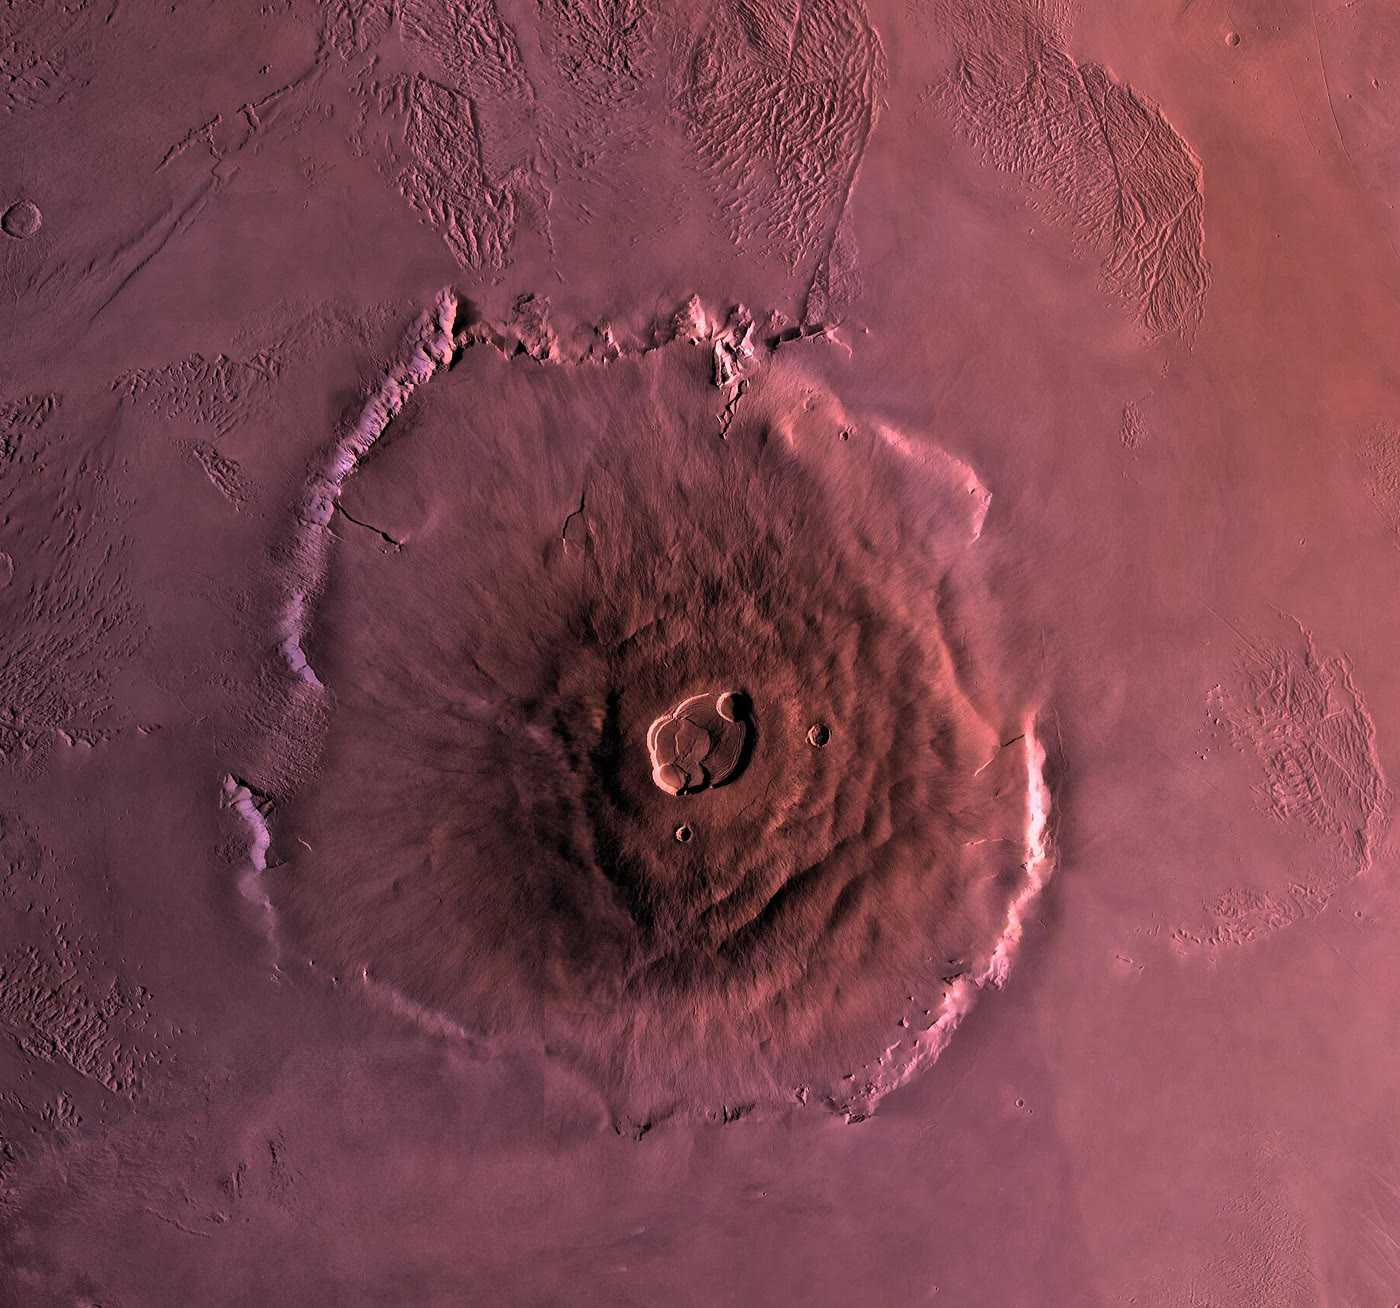
\includegraphics[width=0.48\linewidth]{images/book5/b3-olympus-mons.jpg}
\par\smallskip{\small Olympus Mons di Mars, mosaik citra dari
pengorbit Viking: kaldera puncak di tengah, lereng dengan aliran
lava dan tebing curam yang mengelilingi dasarnya, selebar sekitar \qty{600}{km}.
NASA/JPL/USGS, domain publik.}\label{fig:b3:planetary-interiors-surfaces:olympus}
\end{omfigure}
% ledger: photo:b3-olympus-mons, nasa:olympus-mons

Venus, yang berukuran serupa Bumi, jauh lebih sedikit kawah tumbukannya dibanding
semua planet batuan lain selain Bumi. Permukaannya mungkin memiliki umur rata-rata
semuda 150 juta tahun, dengan bagian yang lebih tua di antaranya:
vulkanisme dan deformasi memperbarui sebagian besar permukaannya, mungkin sedikit demi sedikit
dalam waktu lama, mungkin juga lebih cepat. Venus memiliki ribuan gunung api dan
tidak ada tanda lempeng yang bergerak.
% ledger: nasa:venus-surface, planet:Venus.diameter, planet:Earth.diameter

Io, bulan besar terdekat Jupiter, kehilangan lebih dari
\qty{2.5}{W.m^{-2}} melalui permukaannya, sekitar 27 kali rata-rata Bumi
yaitu \qty{0.092}{W.m^{-2}}. Panasnya bukan berasal dari radioaktivitas:
melainkan dibangkitkan oleh pasang surut.
% ledger: veeder:io-heat, dd10:split

\begin{definition}[Pemanasan pasang surut]\label{def:b3:planetary-interiors-surfaces:tidal-heating}
\emph{Pemanasan pasang surut}\index{pemanasan pasang surut} adalah panas yang dihasilkan di dalam
benda akibat gesekan dari deformasi yang ditimbulkan oleh pasang surut yang berubah-ubah.
Sebuah bulan yang berotasi sinkron pada orbit eksentrik merasakan pasang surut
dari planetnya yang berubah kekuatannya dan berayun bolak-balik selama setiap orbit.
\end{definition}

\begin{proposition}[Daya pasang surut bulan sinkron]\label{prop:b3:planetary-interiors-surfaces:tidal-power}
Sebuah bulan berjari-jari $R$ yang berotasi sinkron, pada orbit dengan gerak rata-rata
$n$ dan eksentrisitas kecil $e$, melepaskan daya
\[
  \dot E = \frac{21}{2}\,\frac{k_2}{Q}\,\frac{(nR)^5}{G}\,e^2 ,
\]
dengan $Q$ adalah faktor kualitas pasang surut bulan, sehingga $k_2/Q$ mengukur
bagian deformasi pasang surut yang hilang sebagai panas.
\end{proposition}

Proposisi ini diterima tanpa pembuktian. Pasang surut yang melepaskan energi juga membulatkan
orbit; Io tetap berorbit elips, dengan eksentrisitas 0.004, karena
tarikan Europa dan Ganymede yang tepat waktunya mengganggunya, periode orbit mereka
yaitu 1.77, 3.55, dan \num{7.15}~hari, yang hampir tepat berbanding
1:2:4 (\cref{exo:b3:planetary-interiors-surfaces:8}). Permukaannya naik
dan turun hingga \qty{100}{m} setiap orbit.
Gunung api menutupi Io dengan lava lebih cepat daripada kawah dapat terbentuk di atasnya; satu model
tentang bagaimana panasnya lolos adalah \omterm{def:b3:planetary-interiors-surfaces:heat-pipe}{vulkanisme pipa panas}, yang akan menjaga
litosfer tebal dan dingin di bawah permukaannya yang membara.
% ledger: nasa:galilean-orbits, beuthe:tidal-power, nasa:io-orbit, nasa:io-facts

\begin{definition}[Samudra bawah permukaan]\label{def:b3:planetary-interiors-surfaces:ocean-world}
Sebuah \emph{samudra bawah permukaan}\index{samudra bawah permukaan} adalah lapisan global
air cair di bawah kulit es bulan atau planet kerdil, yang dijaga tetap cair oleh
panas pasang surut dan radiogenik.
\end{definition}

\begin{definition}[Kriovulkanisme]\label{def:b3:planetary-interiors-surfaces:cryovolcanism}
\emph{Kriovulkanisme}\index{kriovulkanisme} adalah letusan air, air garam pekat
atau cairan dan uap volatil lainnya, alih-alih batuan cair, ke
permukaan es sebuah bulan atau planet kerdil.
\end{definition}

Kulit es Europa, yang diukur oleh radiometer gelombang mikro wahana Juno
di wilayah yang dilintasinya, rata-rata berketebalan sekitar \qty{29}{km};
di bawahnya terbentang samudra asin yang memuat air dua kali lipat seluruh
samudra Bumi. Pada Enceladus, bulan Saturnus yang berdiameter hanya sekitar \qty{500}{km},
wahana Cassini pada 2005 menemukan semburan butiran es dan gas yang keluar dari
rekahan hangat di dekat kutub selatan, dengan kecepatan sekitar
\qty{400}{m.s^{-1}}. Gravitasinya dan goyangan rotasinya menunjukkan
bahwa semburan itu bersumber dari samudra global, di bawah kulit es setebal 20 sampai
\qty{25}{km} rata-rata, dan mungkin hanya 1 sampai \qty{5}{km} di
kutub selatan.
% ledger: jpl:europa-shell, nasa:europa-ocean, nasa:enceladus

\section{Inti besar dan inti kecil}\label{sec:b3:planetary-interiors-surfaces:cores}

Keempat inti yang diukur membentuk keluarga yang janggal. Relatif terhadap jari-jarinya, inti
Bumi mencapai 0.55 jarak ke permukaan dan Mars 0.54;
Bulan 0.19; Merkurius 0.82. Diferensiasi, dalam volume Tahun 2, memisahkan
logam dari silikat di dalam setiap benda, tetapi tidak dapat membuat proporsi
logam begitu berbeda. Tumbukan raksasa dapat melakukannya. Bulan diduga terbentuk
dari puing tumbukan antara benda sebesar Mars dan
Bumi muda sekitar 4.5 miliar tahun lalu, logam benda penumbuk bergabung dengan
inti Bumi, sedangkan Bulan sebagian besar mengumpulkan batuan mantel, maka intinya
kecil. Tumbukan serupa mungkin telah mengupas sebagian besar mantel silikat
Merkurius dan menyisakannya sebagai planet kaya besi yang intinya memenuhi sebagian besar
dirinya. Inti-inti ini, seperti kawah, merekam sejarah tumbukan.
% ledger: data:prem, jpl:insight-interior, nasa:moon-core, agu:mercury-core, french:giant-impacts

\section{Latihan}

\begin{exercise}[$\star$]\label{exo:b3:planetary-interiors-surfaces:1}
Merkurius memiliki massa jenis rata-rata \qty{5429}{kg.m^{-3}}, faktor momen
inersia 0.35 dan jari-jari \qty{2440}{km}. Dengan model dua lapisan dan
mantel \qty{3300}{kg.m^{-3}}, hitung jari-jari relatif inti,
jari-jarinya dalam kilometer dan massa jenisnya.
\end{exercise}

\begin{exercise}[$\star$]\label{exo:b3:planetary-interiors-surfaces:2}
Sebuah proyektil berbatu berdiameter \qty{50}{m}, dengan massa jenis \qty{3500}{kg.m^{-3}},
menumbuk Bumi secara vertikal dengan kecepatan \qty{20}{km.s^{-1}}. Hitung massa dan
energi kinetiknya, dalam joule dan dalam megaton bahan peledak
($\qty{1}{Mt} = \qty{4.2e15}{J}$). Berapa diameter kawah yang diberikan oleh aturan
dua puluh kali diameter proyektil?
\end{exercise}

\begin{exercise}[$\star$]\label{exo:b3:planetary-interiors-surfaces:3}
Pada dataran Mars seluas \qty{100000}{km^2}, dihitung 120 kawah berdiameter \qty{1}{km} dan
lebih. Hitung $N_1$, galat relatifnya, dan \omterm{def:b3:advanced-geochronology:model-age}{umur model}
dataran beserta galatnya.
\end{exercise}

\begin{exercise}[$\star$]\label{exo:b3:planetary-interiors-surfaces:4}
Io, berjari-jari \qty{1821.5}{km}, kehilangan \qty{2.5}{W.m^{-2}}. Hitung
total kehilangan panasnya dan bandingkan dengan Bumi, \qty{47}{TW}, secara total dan
per meter persegi (\qty{0.092}{W.m^{-2}}).
\end{exercise}

\begin{exercise}[$\star\star$]\label{exo:b3:planetary-interiors-surfaces:5}
Mars memiliki massa \qty{6.417e23}{kg} dan jari-jari \qty{3389.5}{km}.
(a)~Hitung massa jenis rata-rata, gravitasi permukaannya, dan $\rho gR$.
(b)~Anggap ia sebagai bola homogen tak termampatkan dengan rigiditas
\qty{67}{GPa}, hitung \omterm{def:b3:planetary-interiors-surfaces:love-number}{bilangan Love} $k_2$. (c)~Nilai terukur adalah
$0.153 \pm 0.017$. Apa yang disimpulkan dari perbandingan itu?
\end{exercise}

\begin{exercise}[$\star\star$]\label{exo:b3:planetary-interiors-surfaces:6}
Di Bumi ($g = \qty{9.8}{m.s^{-2}}$), transisi dari \omterm{def:b3:planetary-interiors-surfaces:crater-morphology}{kawah sederhana} ke \omterm{def:b3:planetary-interiors-surfaces:crater-morphology}{kawah kompleks}
terjadi pada sekitar \qty{4}{km} di batuan kristalin dan \qty{2}{km} di
sedimen. (a)~Dengan anggapan bahwa diameter transisi bervariasi sebagai $1/g$,
perkirakan nilainya di Bulan ($g = \qty{1.62}{m.s^{-2}}$) dan di Mars serta
Merkurius ($g = \qty{3.7}{m.s^{-2}}$); bandingkan dengan \qty{20}{km}
yang teramati di Bulan. (b)~Jika keruntuhan dimulai ketika $\rho gD/3$ melampaui
kekuatan $Y$ batuan, berapa kekuatan yang diberikan transisi kristalin
Bumi, untuk $\rho = \qty{2600}{kg.m^{-3}}$?
\end{exercise}

\begin{exercise}[$\star\star$]\label{exo:b3:planetary-interiors-surfaces:7}
Sebuah permukaan memuat $\num{2.0e-3}$ kawah berukuran \qty{1}{km} atau lebih per
kilometer persegi. Tentukan \omterm{def:b3:advanced-geochronology:model-age}{umur model} permukaan itu dengan fungsi kronologi Mars,
dengan menyelesaikan persamaannya secara numerik. Berapa umur yang akan diberikan fungsi kronologi Bulan
jika dipakai, dan mengapa keduanya tidak boleh saling dipertukarkan?
\end{exercise}

\begin{exercise}[$\star\star$]\label{exo:b3:planetary-interiors-surfaces:8}
Periode orbit Io, Europa, dan Ganymede masing-masing adalah 1.769138, 3.551181 dan
\num{7.154553}~hari. (a)~Hitung rasio periode berurutan.
(b)~Hitung $1/P_I - 3/P_E + 2/P_G$ dan berikan komentar. (c)~Mengapa resonansi
dapat mempertahankan eksentrisitas yang seharusnya dihilangkan pasang surut?
\end{exercise}

\begin{exercise}[$\star\star$]\label{exo:b3:planetary-interiors-surfaces:9}
Io mengorbit Jupiter dalam \num{1.769138}~hari dengan eksentrisitas 0.004.
Hitung daya yang diberikan proposisi daya pasang surut per satuan $k_2/Q$,
dan nilai $k_2/Q$ yang akan memasok kehilangan panas Io dari
\cref{exo:b3:planetary-interiors-surfaces:4}.
\end{exercise}

\begin{exercise}[$\star\star\star$]\label{exo:b3:planetary-interiors-surfaces:10}
Untuk Bulan, $\bar\rho = \qty{3340}{kg.m^{-3}}$ dan $C = 0.394$.
(a)~Tunjukkan bahwa dalam model dua lapisan $\mathrm dx^2/\mathrm dC =
\tfrac52\bar\rho/(\bar\rho - \rho_m)$ pada $\rho_m$ tetap. (b)~Dengan
massa jenis mantel yang memberikan inti $x = 0.19$ adalah \qty{3288}{kg.m^{-3}},
berapa $x$ dan $\rho_c$ jika $C = 0.395$, dan jika $C = 0.393$?
(c)~Apa yang dikatakan hal ini tentang penimbangan inti kecil dengan momen
inersia?
\end{exercise}

\begin{exercise}[$\star\star\star$]\label{exo:b3:planetary-interiors-surfaces:11}
(a)~Untuk 100 kawah, hitung galat pencacahan \omterm{def:b3:advanced-geochronology:model-age}{umur model}
permukaan Mars berumur \qty{1.0}{Ga} dan satu lagi berumur \qty{3.8}{Ga}.
(b)~Tunjukkan bahwa pada bagian linier fungsi kronologi $\sigma_T/T =
1/\sqrt n$. (c)~Mengapa umur permukaan yang tua masih tidak pasti?
\end{exercise}

\begin{exercise}[$\star\star\star$]\label{exo:b3:planetary-interiors-surfaces:12}
Europa, dengan jari-jari \qty{1560.8}{km}, mengorbit dalam \num{3.551181}~hari dengan
eksentrisitas 0.009. (a)~Jika Europa mendisipasikan pasang surut dengan $k_2/Q$ yang sama
seperti Io, berapa bagian daya pasang surut Io yang akan dihasilkannya, dan berapa aliran panasnya?
(b)~Mengapa anggapan itu diragukan untuk bulan dengan \omterm{def:b3:planetary-interiors-surfaces:ocean-world}{samudra bawah permukaan} di bawah esnya?
\end{exercise}

\section{Soal: Dua dataran di Mars}

\begin{problem}[{Soal akhir pekan --- inti Mars dan umur dua
dataran lava rekaan}]
\label{pb:b3:planetary-interiors-surfaces:1}
Mars memiliki massa \qty{6.4169e23}{kg}, jari-jari \qty{3389.5}{km}, dan
faktor momen inersia 0.366. Dua dataran rekaan, A dan B, terletak di
provinsi vulkaniknya; kawah-kawahnya telah dihitung pada citra dengan bin
selebar $\sqrt2$.

\medskip\noindent\textbf{Bagian I --- Inti.}
\begin{enumerate}
\item Hitung massa jenis rata-rata Mars.
\item Dengan model dua lapisan dan massa jenis mantel \qty{3500}{kg.m^{-3}}, hitung
  jari-jari relatif inti, jari-jarinya dalam kilometer, dan
  massa jenisnya.
\item InSight mengukur jari-jari inti \qty{1830}{km}. Massa jenis mantel dan inti apa
  yang kemudian dibutuhkan model dua lapisan?
\item Bandingkan massa jenis inti itu dengan massa jenis inti luar Bumi
  tepat di bawah puncaknya, \qty{9900}{kg.m^{-3}} dalam model acuan Bumi,
  dan jelaskan mengapa nilai yang lebih rendah diharapkan untuk Mars, serta apa lagi
  yang tersirat.
\item \omterm{def:b3:planetary-interiors-surfaces:love-number}{Bilangan Love} bola homogen Mars dengan rigiditas
  \qty{67}{GPa} adalah 0.109; nilai terukurnya 0.153. Pengamatan mana yang lebih dulu
  diperoleh, dan apa yang sudah dikatakannya tentang inti?
\item Kerak Mars berketebalan 20 hingga \qty{37}{km}. Berapa bagian dari
  volume planet yang dikandungnya? Apakah tepat mengabaikannya?
\end{enumerate}

\medskip\noindent\textbf{Bagian II --- Pencacahan kawah pada dataran A.} Dataran A
meliputi \qty{80000}{km^2}. Kawahnya, menurut bin diameter (km):
\begin{center}
\small
\begin{tabular}{lccccccccc}
\hline
bin & 1--1.41 & 1.41--2 & 2--2.83 & 2.83--4 & 4--5.66 & 5.66--8 & 8--11.3 & 11.3--16 & 16--22.6 \\
\hline
dataran A & 38 & 6 & 5 & 3 & 0 & 0 & 0 & 1 & 1 \\
dataran B & 48 & 8 & 31 & 12 & 7 & 2 & 0 & 2 & 2 \\
\hline
\end{tabular}
\end{center}
\begin{enumerate}[resume]
\item Hitung jumlah kumulatif kawah dataran A, mulai dari \qty{1}{km} ke atas.
\item Hitung $N(\qty{1}{km})$ per kilometer persegi dan simpangan
  baku.
\item Fungsi produksi memberikan $F(\qty{2}{km}) = 0.147$ dan
  $F(\qty{1.41}{km}) = 0.355$. Apakah jumlah pada 1.41 dan \qty{2}{km}
  konsisten dengan bentuk fungsi produksi?
\item Apakah dataran A berada dekat \omterm{def:b3:planetary-interiors-surfaces:crater-dating}{massa jenis kesetimbangan kawah},
  \qty{0.072}{km^{-2}} pada \qty{1}{km}?
\item Mengapa bin dipilih dengan lebar $\sqrt2$?
\item Gugus dan rantai kawah kecil dikeluarkan dari pencacahan. Mengapa?
\end{enumerate}

\medskip\noindent\textbf{Bagian III --- Umur model.} Gunakan fungsi
kronologi Mars.
\begin{enumerate}[resume]
\item Hitung \omterm{def:b3:advanced-geochronology:model-age}{umur model} dataran A. Periksa bahwa suku eksponensial
  dapat diabaikan.
\item Hitung galat pencacahannya.
\item Umur berapa yang akan diberikan oleh kronologi Bulan?
\item Dataran B meliputi \qty{120000}{km^2}. Dengan kawahnya yang berukuran
  \qty{2}{km} dan lebih besar, hitung $N(\qty{2}{km})$, kemudian $N_1$, lalu \omterm{def:b3:advanced-geochronology:model-age}{umur modelnya}, dengan
  menyelesaikan persamaan itu secara numerik.
\item Hitung galat pencacahan dari umur tersebut.
\item Bandingkan galat relatif kedua umur itu dan jelaskan
  perbedaannya.
\end{enumerate}

\medskip\noindent\textbf{Bagian IV --- Kawah terkubur pada dataran B.}
\begin{enumerate}[resume]
\item Berapa banyak kawah antara \qty{1}{km} dan \qty{2}{km} yang seharusnya dimiliki dataran B jika
  seluruh permukaannya berumur seperti pada pertanyaan~16? Berapa banyak yang sebenarnya dimilikinya?
\item Misalkan lava mengubur setiap kawah yang lebih kecil dari \qty{2}{km} pada
  saat $T_r$ dan membiarkan kawah yang lebih besar. Hitung $T_r$ dari
  kawah \num{1}--\qty{2}{km}.
\item Hitung galat pencacahan dari $T_r$.
\item Anggap \omterm{def:b3:planetary-interiors-surfaces:crater-morphology}{kawah sederhana} segar di Mars memiliki kedalaman seperlima
  lebarnya (asumsi soal ini). Seberapa tebal lava harus agar mengubur
  kawah \qty{2}{km}, dan mengapa kawah yang lebih besar masih terlihat?
\item Mungkinkah lava dataran B dan lava dataran A berasal dari satu episode
  vulkanisme?
\item Berikan \omterm{def:b3:advanced-geochronology:model-age}{umur model} dataran A, dalam miliar tahun, hingga dua
  angka penting.
\end{enumerate}
\end{problem}
% ledger: nasa:mars, jpl:insight-interior, yoder:mars-k2, data:prem, craterstats:mars-pf, craterstats:mars-cf, craterstats:moon-cf, craterstats:equilibrium
